\subsection{Highlights of Proof of Theorem~\ref{thm:CDDP2}} \label{sec:ddp-polysize}
Here, we highlight only the important parts of the proof of
Theorem~\ref{thm:CDDP2}. The full proof can be found in
Section~\ref{apx:proof_CDDP2}. 
%
We show that $\Pbase$ satisfies DDP even when the size of
the universe $\U$ of size $n_R \cdot \ell$ is polynomial in $\kappa$
with $\ell = \Omega(n_R^3)$, and the secret set $R$ is chosen from the
uniform distribution on $\U$, conditioned on arbitrary leakage on $R$ of
length $L$, where $L \le n_R (\lg \ell - 3 \lg n_R - 2)$.  WLOG, we assume
that the adversary corrupts $P_1$. 

We set $n_R' := n_R/3$; looking forward, it is the size of
a subset $R' \subset R$, each of whose elements has high remaining
min-entropy even after leakage (that we will define in the proof) is
considered.

\subsubsection{Min-hash Graph}
Consider running the min-hash protocol $\Pbase$ with $k$ iterations such
that $k_g$ of them belong to $G_\theta$. For this, we consider all the hash outputs in two different stages and define the following sets:
%
\[ H_1 = \{ h_j(A_{+\xs})\}_{j=1}^k, 
  ~ H_2 = \{h_j(\U \setminus A_{+x^*})\}_{j=1}^k. \] 
%
 Since we are
in the random oracle model, each hash value is chosen uniformly at
random.  For our analysis, we construct the following bipartite graph
$(\mathcal{X},\mathcal{Y},\mathcal{E})$, which we call the {\em min-hash
graph}, based on the sets $A, I$ and $\xs$ along with
the hash functions as follows:

\begin{enumerate}
\item[] \hspace{-2em} {\bf MinhashG$_{H_1}(A, I, \xs, H_2)$: }

\item Set  $\mathcal{X} = \U \setminus A_{+\xs}$. In other words, the
graph considers {\em all potential elements that could be in $R = B\setminus I$}. A
distribution of $R$ is equivalent to a distribution of how to choose
$n_R$ nodes from $\XXX$.
Note that $H_1$ determines $G_\theta$ (based on the hash values of $A$ and $I$).
We set $\YYY = G_\theta$. In other words, $\YYY$ corresponds to all the good
iterations that could potentially positively contribute to the final count. 

\item 
Let $p_j = \min h_j(I)$. Use $H_2$ to determine the set of edges: 
%
\[\mathcal{E} = \{ (i, j): (i, j) \in \XXX \times \YYY \mbox{ and } h_j(x_i) < p_j = \min h_j(I) \}.\]
%
In other words, existence of an edge $(i,j)$ means that if node $i$
belongs to $R$, iteration $j$ will {\em not} contribute to the final
count. 

\item Output the resulting bipartite graph $(\XXX, \YYY, \EEE)$. 
\end{enumerate}
% \linnote{Re-generating the fig 5 to make it visible. }
% \begin{figure}[htb]
%     \centering
%     \begin{minipage}[b]{0.4\linewidth}
%         \centering
%         
\includegraphics[width=0.55\textwidth]{bipartilenew.png}
%         % \vspace{-1em}
%         \caption{Min-hash graph}
%         \label{fig:bigraph}
%     \end{minipage}
%     % \hfill
%     \begin{minipage}[b]{0.53\linewidth}
%         \centering
%         \begin{tabular}{llllllllllll}
%         \hline
%          & 1 & 2 & 3 & 4 & 5 & 6 & 7 & 8 & 9 & 10 & 11 \\\hline
%         $h_1$  & 0.83 & 0.25 & 0.77 & 0.85 & 0.93 & 0.35 & 0.86 & 0.92 & 0.49 & 0.21 & 0.5\\
%         $h_2$  & 0.62 & 0.83 & 0.27 & 0.59 & 0.63 & 0.26 & 0.4 & 0.26 & 0.72 & 0.36  & 0.6\\
%         $h_3$  & 0.68 & 0.11 & 0.67 & 0.29 & 0.82 & 0.3 & 0.62 & 0.23 & 0.67 & 0.35 & 0.7 \\
%         $h_4$  & 0.02 & 0.43 & 0.22 & 0.58 & 0.69 & 0.67 & 0.93 & 0.56 & 0.11 & 0.42 & 0.8\\
%         \hline
%         \end{tabular}
%         \caption{Example Hash Functions}
%         \label{examplehash}
%     \end{minipage}
% \end{figure}

\noindent
\hspace*{-0.45cm}%
\begin{minipage}[b]{0.35\linewidth}
    \centering
    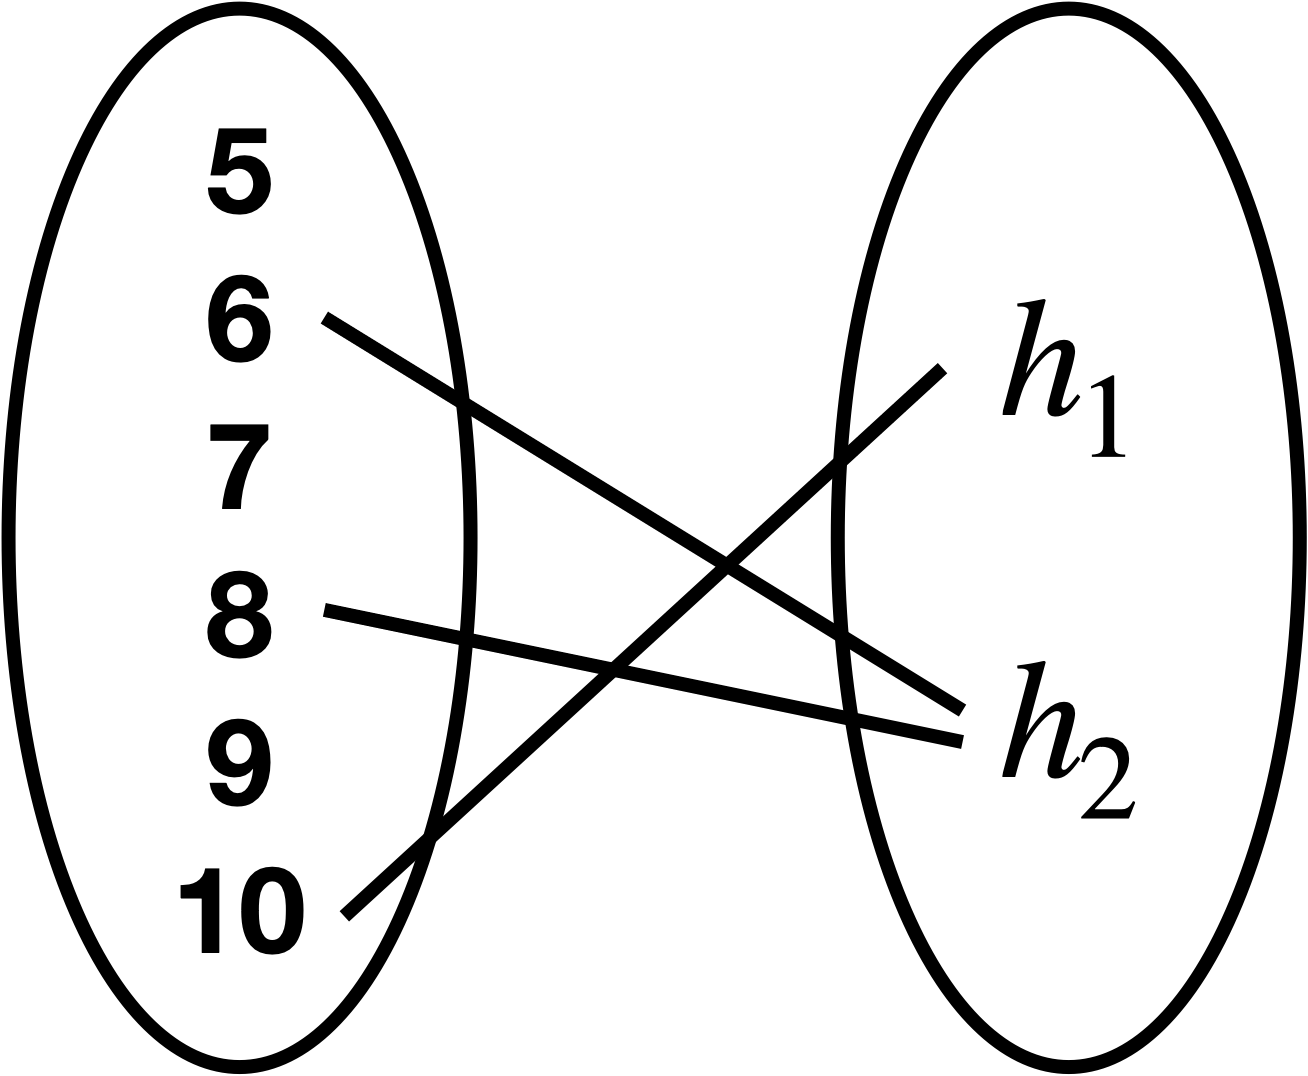
\includegraphics[width=0.55\textwidth]{src/minhash/Images/bipartilenew.png}
    % \vspace{-1em}
    \captionof{figure}{Min-hash graph}
    \label{fig:bigraph}
\end{minipage}%
    % \hfill
\begin{minipage}[b]{0.65\linewidth} \footnotesize
    \centering
    \setlength{\tabcolsep}{3pt}
    \begin{tabular}{llllllllllll}
    \hline
     & 1 & 2 & 3 & 4 & 5 & 6 & 7 & 8 & 9 & 10 & 11 \\\hline
    $h_1$  & 0.83 & 0.25 & 0.77 & 0.85 & 0.93 & 0.35 & 0.86 & 0.92 & 0.49 & 0.21 & 0.5\\
    $h_2$  & 0.62 & 0.83 & 0.27 & 0.59 & 0.63 & 0.26 & 0.4 & 0.26 & 0.72 & 0.36  & 0.6\\
    $h_3$  & 0.68 & 0.11 & 0.67 & 0.29 & 0.82 & 0.3 & 0.62 & 0.23 & 0.67 & 0.35 & 0.7 \\
    $h_4$  & 0.02 & 0.43 & 0.22 & 0.58 & 0.69 & 0.67 & 0.93 & 0.56 & 0.11 & 0.42 & 0.8\\
    \hline
    \end{tabular}
    \captionof{table}{Example Hash Functions}
    \label{examplehash}
\end{minipage}

% \begin{figure}
% \begin{center}
% \includegraphics[width=0.4\textwidth]{bigraph.png}
% \end{center}
% \vspace{-1em}
% \caption{Min-hash graph}
% \label{fig:bigraph}
% \end{figure}

\paragraph{Example.} Let the universe be $\U = [11]$. 
Let $A = \{1, 2, 3, 4\},$ $I = \{2, 3\}$, $\xs = 11$. Let the threshold range for
the $\theta$-good iterations be $[0.2, 0.7]$. Assume that our protocol
runs in 4 iterations using the hash functions defined in table~\ref{examplehash}. %below: 
% \vspace{1em}
% \begin{center}
% \begin{tabular}{llllllllllll}
% \hline
%  & 1 & 2 & 3 & 4 & 5 & 6 & 7 & 8 & 9 & 10 & 11 \\\hline
% $h_1$  & 0.83 & 0.25 & 0.77 & 0.85 & 0.93 & 0.35 & 0.86 & 0.92 & 0.49 & 0.21 & 0.5\\
% $h_2$  & 0.62 & 0.83 & 0.27 & 0.59 & 0.63 & 0.26 & 0.4 & 0.26 & 0.72 & 0.36  & 0.6\\
% $h_3$  & 0.68 & 0.11 & 0.67 & 0.29 & 0.82 & 0.3 & 0.62 & 0.23 & 0.67 & 0.35 & 0.7 \\
% $h_4$  & 0.02 & 0.43 & 0.22 & 0.58 & 0.69 & 0.67 & 0.93 & 0.56 & 0.11 & 0.42 & 0.8\\
% \hline
% \end{tabular}
% \end{center}

Figure~\ref{fig:bigraph} shows the constructed min-hash graph.
%
We have $\XXX = \{5, 6, \ldots, 10\}$ and $\YYY =
\{h_1, h_2\}$; $h_3$ has been ruled out since $p_3 = h_3(2) = 0.11 \not
\in [0.2, 0.7]$, and $h_4$ has been ruled out because $\min h_4(A) \ne
\min h_4(I)$. Moreover, we have $p_1 = h_1(2) = 0.25$ and $p_2 = h_2(3)
= 0.27$. Note that $(8, h_2) \in \EEE$, because $h_2(8) < p_2$.



\subsubsection{Fixed Subsets $(R',T)$ of Secret Items and Good Iterations}
We fix $H_1$ and thereby the nodes $\XXX$ and $\YYY$ of the min-hash
graph.  In this section, as the first step, we fix subsets $R' \subset
\XXX$ and $T \subseteq \YYY$ and analyze the noise over the choice of
$H_2$. In other words, we are treating $H_2$ as private the adversary. Extending
this, in the next section, we will consider the actual protocol setting where
the hash functions are public and then analyze the noise over {\em a
distribution of $R'$}.


\paragraph{Edge distribution in the min-hash graph.}
The probability (over the choice of $H_2$) that an edge $(i,j)$ forms is exactly
equal to $p_j$. Moreover, since we are in the random oracle model, the
probability that $(i,j)$ forms is independent of the probability that any other
edge in the graph forms. 

\paragraph{Noise distribution.}
We are interested in {\em the probability $E^{R'}_{T,r}$ over the
choice of $H_2$ that the final count is reduced by exactly
$r$ due to the elements of $R'$ over a bundle $T$ of iterations.} 
In the random oracle model, the probability depends only on the size of the sets
$n' = |R'|$ and $k_b = |T|$. Therefore, we will often use
the notation $E^{n'}_{k_b,r} = E^{R'}_{T,r}$. We will sometimes even omit
$k_b$ and write $E^{n'}_r$. 
%
Observe that $E^{n'}_{r}$ is another way of representing an
Additive Poisson Binomial distribution. That is, 
%
$E^{n'}_{k_b,r} = \Pr[ \PB(k_b, p_J) = r ].$
%
Therefore, based on Lemma~\ref{lem:pb-dp}, we have the following: 
%
\begin{corollary} \label{lem:concrete_expected_probs}
Let $k_b \in \Omega(\kappa)$, and consider any $H_1$ that makes $|\YYY| >
k_b$ in the min-hash graph construction. For any $s = O(\lg\lg\kappa)$, any
constant $\ee$, there are $a, b \in [k_b]$ such that over the choice of $H_2$,
we have \begin{itemize}
\item For any $r \not \in[a + s, b]$, then $E^{n_R'}_{k_b, r}$
  and $E^{n_R'}_{k_b, r-s}$ are both negligible in $\kappa$.
\item For any $r \in [a, b]$, then it holds  
$e^{-\ee/3} \leq E^{n_R'}_{k_b, r}/E^{n_R'}_{k_b, r-s}
\leq e^{\ee/3}$.
\end{itemize}
\end{corollary}


The above indicates that the distribution over $r$ is amenable for use as a
noise distribution in a differential privacy context. 


\subsubsection{Noise Over the Choice of $R'$ with Public Hash Functions} 
Our main technical challenge is to show that the properties needed for
differential privacy hold {\em even when the hash functions are public}. 

For this, we first fix $H_1$ and $H_2$. Then, we consider the derived min-hash graph $G =
(\XXX, \YYY, \EEE)$. 
Let  $\DDD$ be the distribution of $R'$.
For any set $T$ of iterations of size $k_b$ and any
integer $r$, let $I_{R', T, r}$ be the indicator random variable that is set to
$1$ if set $R'$ contributes $-r$ to the total count in the min-hash protocol. 
%
We define a random variable $D_{T,r}$ that is \emph{the probability that $R'$ contributes to the noise reduction $r$ over iterations in
$T$}: %
\[ D_{T,r}(\DDD) := \Pr_{R' \sim \DDD}[ I_{R', T, r} ] = 
\sum_{R'} \Pr_{R' \sim \DDD}[R'] \cdot I_{R', T, r}. \]


\paragraph{Conditions for the hash functions.}
Ideally, we would like to show the following:
\begin{itemize}
    \item[]  For any fixed $H_1$ and $H_2$ and over distribution $\DDD$, it holds that $D_{T, r}$ and $D_{T, r-1}$ (and ultimately $D_{T, r-s}$) are close, except with the tail case of $r$ whose  probability weight is negligible.   
\end{itemize}

The universal quantifier for $H_1$ and $H_2$ in the above can be
{\em slightly relaxed so that the condition holds with all but small
probability over the choice of the hash functions}, which can be captured
by showing that $D_{T,r}$ is close to its mean $E_{\hat k,r}^{n_R'}$
(and then applying Corollary~\ref{lem:concrete_expected_probs}). 
%


\paragraph{Geometric collision property.}
This is essentially to show that $D_{T,r}$ is strongly concentrated around its
mean. We could try to apply Chernoff bound to show the concentration
property, but we cannot do so because $I_{R'_i, T, r}$ and $I_{R'_j, T, r}$
are not necessarily independent if $R'_i \cap R'_j \neq \emptyset$.
Therefore, we instead use Chebyshev for bounding the tail, which
requires $D_{T,r}$ to have small variance.  Thus, our next goal is to
upperbound $\mathsf{Var}[D_{T,r}]$.
%
To do so, we introduce a property of distributions $\mathcal{D}$ over
sets $R'$ which we call the ``Geometric Collision Property''.  In a
nutshell, this property states that the probability that two sets $R'_1,
R'_2$ drawn independently from $\mathcal{D}$ have intersection of size
$z$ is at most 
$(\frac{1}{n^{0.5}})^z$ for all $z \in [n']$.  We show that
$\mathsf{Var}[D_{T,r}]$ can be bounded for any distribution over sets $R'$
that has this property.


\begin{definition}[Geometric Collision Property]\label{def:geo_col} Let
$\mathcal{D}$ be a distribution over sets $R'$ of size
$n'_R$.  We say that ${\mathcal{D}}$ has the \emph{Geometric Collision
Property} if for all $z \in [n'_R]$
\[
\Pr_{R'_i, R'_j \sim {\mathcal{D}}} \left [|R'_i \cap R'_j| = z \right ] \leq \left ( \frac{1}{\sqrt{n_R}} \right)^z.
\]
\end{definition}

Based on this property, we can show the following lemma. 
%
\begin{restatable}{lemma}{lfixedoracle} \label{cor:fixed_oracle_prob}
Let $k_b \in \Omega(\kappa)$, and consider any $H_1$ that makes $|\YYY| >
k_b$ in the min-hash graph construction. 
Let $\DDD$ be a distribution over sets of size $n_R'$ with geometric
collision property. 
For any set $T$ of size $k_b \in \Omega(\kappa)$, there exist $a, b \in [k_b]$, such that with probability
$1-O(\frac{k_b \cdot \lg^3(\kappa)}{\sqrt{n_R}})$ over choice of $H_2$, the following holds:
\begin{itemize}
    \item For all $r \not \in [a+s, b]$, $D_{T,r}$ is negligible, where $s = O(\lg\lg \secparam)$.
    \item For all $r \in [a, b]$, $e^{-\epsilon/3} E^{n'_R}_{k_b,r} \leq D_{T,r} \leq e^{\epsilon/3} E^{n'_R}_{k_b,r}$.
\end{itemize}
\end{restatable}

The proof is found in Section~\ref{sec:fixed_oracle_prob}. 

\paragraph{Multiple bundles of iterations towards DDP with negligible $\delta$.}
We are not quite done yet. Using the above lemma, we are only able to
reduce the failure probability only to $\sim 1/\sqrt{n}$, whereas we
would like the failure probability to be negligible.  In order to do
that, we split the ``good'' iterations into $u$ bundles, where $u$ is a
small superconstant number $u = \lg\lg \secparam$, and argue that
with overwhelming probability at least one bundle serves as a good noise. Note
that hash outputs are independent in each bundle and so the probability
that all $u$ bundles fail should be $~(\frac{1}{\sqrt{n}})^u$, which is
negligible. For this, we set the parameter $k_b = k_g/u$, where $k_g$ is the
number of good iterations. 
%over choice of $R'$ is good for at least one bundle (with all but negligible
%probability) is sufficient to complete the proof of distributional differential
%privacy. 



\subsubsection{Geometric Collision Property In the Face of Leakage}
We conclude the proof by showing that $R'$ indeed has the geometric collision
property. It is not hard to see that the uniform distribution over all sets $R'$
of size $n'$ from a universe of size $n' \cdot \ell$ (where $\ell \in
\Omega(n^3)$) satisfies the ``Geometric Collision Property''.  It would seem,
therefore, that we could take this as our secret distribution and the analysis
would be complete. Unfortunately, even for the case in which the distribution is
sets of size $n'$ chosen uniformly at random from the universe, the analysis is
not straightforward. The difficulty stems from the fact that the ``noise'' in
the protocol is tied to the input itself. Therefore, if information about the
input is leaked in any other part of the protocol, then the noise distribution
changes and may no longer satisfy the required properties.  Specifically in our
case, learning the number of matches across the two parties' sets with respect
to some of the hash functions leaks information about the secret set of the
honest party (since the secret set affects those counts).

\paragraph{Strong chain-rule for min-entropy.}
We first observe that our initial min-entropy in the distribution over
secret sets $\mathcal{R}$ is high (approximately $\frac{8n}{9} \lg \ell + 2n$) and that
the entire information leaked about $R$ from the counts of the
iterations that are not $\theta$-good is small.  We can lower-bound the
remaining min-entropy in $\mathcal{D}$, therefore, using the weak chain
rule for min-entropy~\cite[Lemma 2.2]{DORS08}.

If we want to use the weak chain rule to  lower bound the remaining min-entropy
with all but $2^{-\kappa}$ probability, however, we need to take a hit of
$\kappa$ in the min-entropy. %
Recall that each individual element in $R$ can be viewed as being chosen
from a set of size $\ell$ and thus has min-entropy of at most
$\lg(\ell) \ll \kappa$.  Thus, after applying the weak chain rule and
losing more than $\kappa$ bits of min-entropy, we can have certain
elements that have only constant min-entropy, thus implying that
collisions are likely in those positions. So the weak chain rule, while leaking only a
small number of bits overall, can ruin the geometric collision property.
Even worse, the min-entropy definition doesn't rule out the case in
which \emph{all} elements of $R$ (i.e.~the marginal distributions over
each element in $R$) have only constant min-entropy, while the total
min-entropy in $R$ remains high!

This phenomenon has been previously observed and studied in the
literature~\cite{skorski2019strong}. One way to deal with such a counter-intuitive
situation is to actually leak a small amount of \emph{additional}
information, known as ``spoiled'' bits. This will lower the total
min-entropy in $R$, but will ensure that a large fraction of blocks in
$R$ still have high min entropy of at least $1.5\lg(n)$. We extend the
techniques of \cite{skorski2019strong} to produce spoiling leakage so that the min-entropy
in $R$ still stays high in our protocol. We discuss more details about the
strong chain rule in the next section. 
